
\chapter{Үйлдлийн тооллын үндэс} \index{Үйлдлийн тоолол}
\section{Лапласын хувиргалт. Уг эх ба дүрслэл} \index{Уг эх}
\begin{thm}
 $f:\mathbb{R}\rightarrow \mathbb{C}$ функцийн хувьд
 \begin{enumerate}
     \item $t<0$ үед $f(t)\equiv 0,$
     \item $t\geq 0$ үед $f(t)$ функц нь хэсэгчилсэн тасралтгүй ба дурын битүү интервал дээр төгсгөлөг ширхэг 1-р төрлийн тасралттай.
     \item $\exists M>0$, $\tilde{a}>0$ ба $\forall t>0$ хувьд $|f(t)|\leq Me^{\tilde{a}t} (inf \tilde{a}=a)$ тоог $f$-н өсөлтийн зэрэг гэдэг) нөхцөлүүд биелж байг.
     
     Тэгвэл
     \begin{eqnarray} \label{10.1}
      F(z)=\int\limits_0^{+\infty} e^{-zt}f(t)
     \end{eqnarray}
     функцийн хувьд
     \begin{enumerate}
         \item [a)] $\re z<0$ мужид утгагүй (интервал сарнина)
         \item [б)] $F(z)\in H (\{\re z>a)\}$ байна. 
         \item[В)] $\forall a_0>a$ хувьд $\re z\geq a_0$ мужид уг интервал жигд нийлнэ.
     \end{enumerate}
 \end{enumerate}
\end{thm}
\begin{dfn}
$f(t)$ функцийг уг эх, $F(z)$ функцийг дүрслэл \index{Дүрслэл}гээд энэ харгалзааг Лапласын хувиргалт \index{Лапласын хувиргалт} гэж нэрлэгдэх ба $\ml{f(t)}=F(z)$ тэмдэглэл хэрэглэдэг.
\end{dfn}
\section{Лапласын хувиргалтын чанарууд} 
Хэрэв $\ml{f(t)}=F(z)$ байвал 
\begin{enumerate}
    \item $\ml{\sum\limits_{k=1}^n a_k f_k(t)}=\sum\limits_{k=1}^n a_kF_k (z)$ (шугаман чанар). 
    \item $\ml{f(at)}=\dfrac{1}{a}F\left(\dfrac{z}{a}\right).$
    \item $f_\tau (t) = \begin{cases}
     0, \qquad \tau >t \\
     f(t-\tau), \qquad \tau \leq t
    \end{cases}$ бол $\ml{f_\tau}=e^{-\tau z}F(z.)$
    \item $\ml{f'(t)}=zF(z)-f(0)$
    \item $\ml{f^{(n)}(t)}=z^n\left(F(z)-\dfrac{f(0)}{z}-\dfrac{f'(0)}{z^2}-\cdots -\dfrac{f^{(n-1)}(z)}{z^n}\right).$
    \item $\ml{\int\limits_0^t f(\tau)d\tau}=\dfrac{1}{z}F(z)$
    \item $\ml{\int\limits_{0}^t f_1(\tau) \cdot f_2(t-\tau)d\tau}= F_1(z)\cdot F_2(z)$
    \item $\ml{(-1)^nt^n\cdot f(t)} = F^{(n)}(z)$
    \item $\ml{\int\limits_{z}^\infty F(z)dz}=\dfrac{f(t)}{t}$
    \item $\ml{e^{-\lambda t}f(t)}=F(z+\lambda)$
\end{enumerate}
чанарууд биелдэг.

Эдгээр чанарууд нь (\ref{10.1}) томьёоноос параметр агуулсан интегралыг хувиргах замаар гаргаж ирдэг. Жишээ болгож 7-р чанарыг баталъя.
\begin{align*}
    F'(z)&=\left(\int\limits_0^{+\infty} e^{-zt}f(t)dt\right)'=\int\limits_0^{+\infty} (e^{-zr})'_zf(t)dt=\\
    &=\int\limits_{0}^{+\infty} \ml{e^{-zt}(-tf(t))dt}= -tf(t)
\end{align*}
Лапласын хувиргалт нь ердийн дифференциал ба интеграл тэгшитгэлүүдийг ердийн тэгшитгэлд шилжүүлэх тухайн уламжлалт дифференциал тэгшитгэлийг ердийн дифференциал тэгшитгэлд шилжүүлэх зэргээр ашигладаг.
\begin{exm}
$
\begin{cases}
 y'+y=1 \\
 y(0)=0
\end{cases}$ байг. $\ml{y(x)}=F(z)$ гэвэл 4-р чанар ёсоор  
\end{exm}
\begin{prf}
$\ml{y'}=zF(z)-0$ ба томьёо 10.1 ёсоор $\ml{1}=\dfrac{1}{z}$ тул $zF(z)+F(z)=\dfrac{1}{z}$ болно. 
\begin{equation} \tag{$*$} \label{10*}
 F(z)=\ml{\frac{1}{z(z+1)}}=1-e^{-z}
\end{equation} энэ томьёог (\ref{10.1})-ээр шалгана уу.

Иймд $y(x)=1-e^{-x}$. Үүнээс харвал дүрслэлээр нь уг эхийг олох аргачлал шаардагдаж байна. Энд дээрх чанарууд ба нэгэнт бодогдсон Лапласын хувиргалтын хүснэгтийг ашиглаж болно. 

Лапласын хувиргалтын хүснэгт 
\begin{enumerate}
    \item $\ml{1}=\dfrac{1}{z}$
    \item $\ml{t^n}=\dfrac{\Gamma (n+1)}{z^{n+1}}, \qquad (n>-1)$
    \item $\ml{e^{at}}=\dfrac{1}{z-a}$
    \item $\ml{\sin at}=\dfrac{a}{z^2+a^2}$
    \item $\ml{\cos at}=\dfrac{z}{z^2+a^2}$
    \item $\ml{\sh at}=\dfrac{a}{z^2-a^2}$
    \item $\ml{\ch at}=\dfrac{z}{z^2+a^2}$
    \item $\ml{t^ne^{at}}=\dfrac{n!}{(z-a)^{n+1}}, \quad (n\in\mathbb{N})$
\end{enumerate}
Одоо энэ хүснэгтийг хэрхэн ашиглаж (\ref{10*}) томьёог гарган авч байгааг харъя.
$$\frac{1}{z(z+1)}=\ml{\frac{1}{z}-\frac{1}{z+1}}=1-e^{-t}$$
(энд 1 ба 3 томьёо ба чанар 1 ашиглагдсан болно). Дүрслэлээр уг эхийг олох ерөнхий томьёо нь голоморф функцийн интеграл ашигладаг ба энэ талаар 10.3-д үзнэ.
\hfill $\blacksquare$\end{prf}
\section{Меллиний томьёо}\index{Меллиний томьёо}
\begin{thm}
 $f(t)$ нь хэсэгчилсэн гөлгөр, $a$ өсөлтийн зэрэгтэй уг эх байг. $F(z)$ нь түүний дүрслэл гэвэл $\forall t>a$ бол 
 $$f(t)\doteq \frac{1}{2\pi i}\int\limits_{x-i\infty}^{x+i\infty} e^{zt}F(z)dz$$
 (энд $x:x>a$ байх дурын бодит тоо) (энд $\doteq$ Фурьеийн тэнцэтгэл, тасралтгүй цэгүүд дээр тэнцэнэ).
\end{thm}
\begin{prf}
$x>a$ байг.
\begin{equation} \tag{$*$} \label{11*}
    \varphi (t)=e^{-xt} f(t)
\end{equation}
функц хэсэгчилсэн гөлгөр ба $x\rightarrow +\infty$ үед экспонент хурдаар тэг рүү тэмүүлэх ёстой. Иймд Фурьегийн интеграл ашиглавал
$$\varphi (t)\doteq \frac{1}{2\pi} \int\limits_{\infty}^{+\infty} d\xi \int\limits_{-\infty}^{+\infty} \varphi (\eta) e^{i\xi (t-\eta)} d\eta$$
байна. Энд (\ref{11*}) томьёог тавивал 
$$e^{-xt}f(t)\doteq \frac{1}{2\pi} \int\limits_{-\infty}^{+\infty} e^{i\xi}d\xi \int\limits_{0}^{+\infty}  e^{-(x+i\xi)\eta } f(\eta)f(\eta)d\eta$$
байна. 
$$x+i\xi =z \quad \text{гэвэл} \quad \int\limits_0^{+\infty} e^{-(x+i\xi)\eta}f(\eta) d\eta =F(z) \quad \text{учир}$$
$$f(t)\doteq \frac{1}{2\pi}\int\limits_{-\infty}^{+\infty} e^{(x+i\xi)t} F(z)d\xi =\frac{1}{2\pi i}\int\limits_{x-i\infty}^{x+i\infty} e^{zt}F(t)F(z)dz$$
Иймд Меллиний хувиргалт нь Фурьегийн утгаар Лапласын хувиргалтын урвуу болж болно.
\hfill $\blacksquare$\end{prf}
\begin{thm}
 $F(z)\in H(\{\re z>a\})$ хувьд 
 \begin{enumerate}
     \item [a)] $|z|\rightarrow \infty$ үед $F(z)$  утга жигд тэг рүү тэмүүлж байг.
     \item [б)] $\forall x>a$ хувьд $\bint\limits_{x-i\infty}^{x+i\infty} |F(z)|dy$
жигд нийлдэг байг.

Тэгвэл $F(z)$ нь  $f(t)=\dfrac{1}{2\pi i}\bint\limits_{x-i\infty}^{x+i\infty} e^{zt}F(z)dz(z>a)$ функцийн дүр байна.
 \end{enumerate}
\end{thm}
\section{Меллиний томьёог хэрэглэх нь}
\begin{exm}
$\ml{f_1(t)}=F_1(z)$; $\ml{f_2(t)}=F_2(z)$ бол 
$$\ml{f_1(t)\cdot f_2(t)}=\frac{1}{2\pi i}\int\limits_{x-i\infty}^{x+i\infty} F_1(\zeta)\cdot F_2(z-\zeta)d\zeta $$
\end{exm}
\begin{sol}
\begin{align*}
    \ml{f_1(t) \cdot f_2(t)}&=\int\limits_0^\infty e^{-zt}f_1(t)f_2(t)dt \\
    &=\int\limits_0^\infty e^{-zt}\left(\frac{1}{2\pi i} \int\limits_{x-i\infty}^{x+i\infty} e^{\zeta t}F_1(\zeta)d\zeta \right) \cdot f_2(t)dt \\
    &=\frac{1}{2\pi i}\int\limits_0^\infty \int\limits_{x-i\infty}^{x+i\infty} e^{(\zeta-z)t}F_1(\zeta)f_2(t)d\zeta dt \\
    &=\frac{1}{2\pi i} \int\limits_{x-i\infty}^{x+i\infty} F_1(\zeta)\left(\int\limits_0^\infty e^{(\zeta -z)t}f_2(t)dt\right) d\zeta \\
    &=\frac{1}{2\pi i} \int\limits_{x-i\infty}^{x+i\infty} F_1(\zeta)F_2(\zeta-z)d\zeta.
\end{align*}
\end{sol}
\begin{exm}
$f_1(t)=\cos at$, $f_2(t)=t$ бол $f(t)=t\cos at$ дүрийг ол.
\end{exm}
\begin{sol}
$\ml{\cos at}=\dfrac{z}{z^2+a^2}$ $\ml{t}=\dfrac{1}{z^2}$ тул Жишээ 10.2 ёсоор 
$$F(z)=\frac{1}{2\pi i}\int\limits_{x-i\infty}^{x+i\infty} \frac{\zeta}{\zeta^2+a^2}\cdot \frac{1}{(\zeta -z)^2}d\zeta$$
 Зурагт үзүүлсэн контураар интегралчилбал хагас тойргийн дагуух интегралын утга радиус өсөхөд тэг болохыг харуулж болно. 
 \begin{center}
     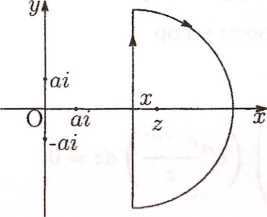
\includegraphics[width=5cm]{Zurag/43.jpg}
 \captionof{figure}{}
        \label{ref hiih ner}
 \end{center}

Иймд
\begin{align*}
    (z)&=\frac{1}{2\pi i}\left(-2\pi i 
    {\tiny{\begin{array}{c}
Res  \\
 \zeta =z
\end{array}}}
    \frac{\zeta}{(\zeta^2+a^2)(\zeta -z)^2}\right) \\
    &=-\frac{d}{d\zeta}\left(\frac{\zeta}{\zeta^2+a^2}\right)\Big |_ {\zeta =z}=\frac{z^2-a^2}{(z^2+a^2)^2}
\end{align*} Иймд $\ml{t\cdot \cos at}=\dfrac{z^2-a^2}{(z^2+a^2)^2}$
\end{sol}
\begin{exm}
$F(z)=\dfrac{e^{a\sqrt{z}}}{z}$-функцийн эхийг ол.
\end{exm}
\begin{sol}
$\mathbb{C}$ хавтгайг $(-\infty, 0]$ дагуу огтлол хийсэн гээд энэ муж дээр $z>0$ үед $\sqrt{z}>0$ байх мөчрийн аналатик үргэлжлэлийг авч үзье.
\begin{center}
     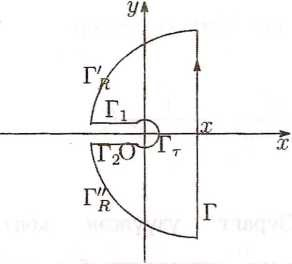
\includegraphics[width=5cm]{Zurag/44.jpg}
 \captionof{figure}{}
        \label{ref hiih ner}
\end{center}
 Зурагт үзүүлсэн хэрчим ба тойргийн нумуудаар (радиус нь $R$, $r$ байх) хүрээлэгдсэн контур авч үзье. Кошийн теорем ёсоор
$$\left(\int\limits_{\Gamma}+\int\limits_{\Gamma'_R\wedge \Gamma''_R}+\int\limits_{\Gamma_1\wedge \Gamma_2}+\int\limits_{\Gamma_\tau}\right) \left(e^{zt}\frac{e^{-z\sqrt{z}}}{z}\right)dz=0$$ байна. 

Одоо $R\rightarrow \infty$, $r\rightarrow 0$ гэвэл 
\begin{align*}
    &\int\limits_{\Gamma} e^{zt}\dfrac{e^{-a\sqrt{z}}}{z}dz\rightarrow 2\pi i f(t) \qquad \text{(Меллиний хувиргалт)} \\
     &\int\limits_{\Gamma'_R\wedge \Gamma''_{R}} e^{zt}\dfrac{e^{-a\sqrt{z}}}{z}dz\rightarrow 0 \qquad \text{(Жорданы лемм)}
\end{align*}
$$\int\limits_{\Gamma_\tau} e^{zt}\frac{e^{-a\sqrt{z}}}{z}dz=\lim\limits_{\varepsilon \rightarrow 0}\int\limits_{-\pi +\varepsilon}^{\pi -\varepsilon} e^{rte^{i\varphi}}\frac{e^{-a\sqrt{r}e^{i\frac{\varphi}{2}}}}{re^{i\varphi}}\cdot ure^{i\varphi} d\varphi \xrightarrow[r\rightarrow 0]{}\int\limits_{-\pi}^\pi id\varphi=2\pi i$$
байна. 
\begin{align*}
    \int\limits_{\Gamma_1\wedge \Gamma_2}e^{zt}\frac{e^{-a\sqrt{z}}}{z}dz &\xrightarrow[]{} -\int\limits_0^\infty \frac{e^{-yt}e^{-ia\sqrt{y}}}{y}dy+\int\limits_0^\infty \frac{e^{-yt}e^{ia\sqrt{y}}}{y}dy\\
    &=2\pi i \int\limits_0^\infty \frac{e^{-yt}}{y}\sin a\sqrt{y}dy
\end{align*}
 байна. 

Иймд $f(t)=1-\dfrac{1}{\pi}\int\limits_0^\infty e^{-yt}\frac{\sin a\sqrt{y}}{y}dy$ гэсэн дүрсээр эхийг олно. Френелийн интеграл ашиглан
$$f(t)=1-\Phi \left(\frac{a}{2\sqrt{t}}\right) \qquad \left(\text{энд} \quad \Phi(t)=\frac{2}{\sqrt{\pi}}\int\limits_0^t e^{-y^2}dy\right)$$
болохыг харуулж болно.
$$\ml{\frac{e^{-a\sqrt{z}}}{z}}=1-\Phi \left(\frac{a}{2\sqrt{t}}\right)$$
\end{sol}
\begin{exm}
$F(z)=\sum\limits_{n=1}^\infty \dfrac{a_n}{z^n}$ бол 
$$
\ml{F(z)}=f(t)=
\begin{cases}
 0, \qquad t<0 \\
 \sum\limits_{n=0}^\infty C_{n+1}\frac{t^n}{n!}, \qquad t>0
\end{cases}
$$ 
\end{exm}
\begin{sol}
$\ml{\dfrac{t^n}{n!}}=\dfrac{1}{z^{n+1}}$ тул шугаман чанар ёсоор 
$$\ml{\sum\limits_{n=0}^\infty C_{n+1}\frac{t^n}{n!}}=\sum\limits_{n=0}^\infty C_{n+1}\frac{1}{z^{n+1}}=F(z)$$ батлагдав. 
\end{sol}
\begin{exm}
$$\frac{e^{-\frac{1}{z}}}{z}=\mathcal{L}\left\{\sum\limits_{n=1}^\infty \frac{(-1)^{n-1}}{(n-1)!\cdot z^n}\right\}=\sum\limits_{k=0}^\infty (-1)^k \frac{\left(\frac{2\sqrt{t}}{2}\right)^{2k}}{(k!)^2}=J_0(2\sqrt{t})$$
(Энд $J_0$ Бесселийн тэг эрэмбийн функц).
\end{exm}
\begin{exm}
$$y^{IV}+2y''+y=0$$
$$y(0)=y'(0)=y''(0)=0$$
$$y'''(0)=1 \quad \text{бод}.$$
\end{exm}
\begin{sol}
Хэрэв $\ml{y}=F(z)$ гэвэл  \\
$\ml{y^{IV}}=z^4\left(F(z)\dfrac{1}{z^4}\right) =z^4F(z)-1$\\
$\ml{y''}=z^2F(z)$ тул $z^4F(z)-1+2z^2F(z)+F(z)=0\Rightarrow $\\
$F(z)=\dfrac{1}{z^4+2z^2+1}$ байна. Иймд Меллиний томьёо ёсоор 
$$y(x)=\frac{1}{2\pi i}\int\limits_{t-i\infty}^{t+i\infty} e^{zx}\frac{dz}{z^4+2z^2+1}$$
Зурагт үзүүлсэн контурыг ашиглавал $\Gamma_R$ хувьд жорданий лемма хүчинтэй тул
$$y(z)= {\tiny{\begin{array}{c}
Res  \\
 \zeta =z
\end{array}}} \frac{e^{zx}}{(z+i)^2}+ {\tiny{\begin{array}{c}
 Res  \\
 \zeta =z
\end{array}}}\frac{e^{zx}}{(z-i)^2}=\frac{1}{2}(\sin x-x\cos x)$$
\end{sol}
\begin{exm}
$
\begin{cases}
 y''\neq y=\sin t \\
 y(0)=0 \\
 y'(0)=0
\end{cases} 
$ бод. 
\end{exm}
\begin{sol}
$z^2F(z)+F(z)=\dfrac{1}{z^2+1} \Rightarrow F(z)=\dfrac{1}{(z^2+1)^2}.$\\ Иймд
$y(x)=\dfrac{1}{2\pi i}\bint\limits_{t-i\infty}^{t+i\infty} e^{zx}\cdot \dfrac{1}{(z^2+1)^2}dz=\dfrac{1}{2}(\sin x-x\cos x).$
\end{sol}
\begin{exm}
$\begin{cases}
 u_t=a^2u_{xx}\\
 u(x,0)=0\\
 u(0,y)=q(t)
\end{cases} 
$ \\
тухайн уламжлалт дифференциал тэгшитгэлийг бод. $x$ бэхлээд $t$ хувьд Лапласын хувиргалт хийвэл
\begin{align*}
    \ml{u(x,t)}=U(x,z)\\
    \ml{u_t(x,t)}=zU(x,z)\\
    \ml{u_{xx}(x,t)}=U_{xx}(x,z)
\end{align*} тул 
$$\begin{cases}
 U_{xx}(x,z)+\dfrac{z}{a^2}U(x,z)=0\\
 U(0,z)=Q(z)
\end{cases}
$$ болж энгийн дифференциал тэгшитгэл үүсэх рүү шилжинэ.
$$U(x,z)=Q(z)\cdot e^{-\frac{\sqrt{z}}{a}x}$$ тул 
$$u(x,t)=\frac{1}{2\pi i}\int\limits_{t-i\infty}^{ti\infty} e^{zx}Q(z)e^{-\frac{\sqrt{z}}{a}x}dz$$ байна.
\end{exm}
\begin{center}
    \textbf{Дасгал}
\end{center}
$F(z)=\dfrac{w}{z^2+w^2}, \quad \re z>0$ бол дүрийг ол. 
\\
\newpage
\begin{center}
    \textbf{Ашигласан ном зохиол}
\end{center}
\begin{enumerate}
    \item Гурвиц А., Курант Р. Теория функций (Перев.с Нем.с Евграпова М.А.) “Наука”, М., 1968.
    \item Привалов И.И. Введение в теорию функций комп- лексного переменного, изд.12-ое “Наука”, М., 1977.
    \item Маркушевич А.И. Краткий курс теории аналити- ческих функций, “Наука”, М., 1978.
    \item Шабат Б.В. Введение в комплексный анализ. ч.I, Функции одного переменного ч.II. Функции нескольких переменных, изд.З-е, “Наука”, М., 1985.
    \item Стоилов С. Теория функций комплексного переменного, т.I, т.II, перев.с Рум. Берштейна И., ИЛ, М., 1962.
    \item Евграфов М.А. Аналитические функции, “Наука”, М., 1965
    \item Бицадзе А. В Основы теории аналитических функций комплексного переменного, “Наука”, М., 1969.
    \item Свешников А,Г., Тихонов А.Н. Теория функций комплексной переменной, “Наука”, М., 1967
    \item Волковыский Л.И., Лунц Г.Л., Араманович И.Г. Сборник задач по теории функций комплексного переменного, изд.2-е, “Наука”, М.,1970
\end{enumerate}